\chapter{Design}\label{chap:design}

\section{Emulator}

\subsection{Zentrale Struktur}

\begin{listing}[ht]
\begin{minted}{rust}
    struct Emulator {
        pc: u16,
        sp: u16,
        ram: RAM,
        reg: RegisterArray,
        input_devices: [InputDevice; 256],
        output_devices: [OutputDevice; 256],
        running: bool,
        interrupts_enabled: bool
    }
\end{minted}
\centering
\caption{Zentrale Emulator Struktur}
\label{lst:wtf}
\end{listing}

Den Kern des Emulators bildet eine Struktur, welche zuständig für die Ausführung der Maschinencode-Programme ist. Diese Struktur gruppiert alle notwendigen Komponenten eines Intel 8080 Systems. Der Aufbau der Struktur ist in \cref{lst:wtf} illustriert.

Diese Komponenten wurden in \cref{chap:prereqs} bereits erklärt: \rust{pc} und \rust{sp} sind 2 16-Bit-Zahlen, die den Program Counter und den Stack Pointer repräsentieren. \rust{ram} ist der Arbeitsspeicher und \rust{reg} simuliert die Register (inklusive Flags und Akkumulator).
Die Ports für I/O-Geräte werden durch 2 Arrays mit jeweils 256 Elementen repräsentiert.
Darauf folgt ein Boolean, die aussagt ob der Emulator am Laufen ist und der Boolean die anzeigt ob Interrupts erlaubt sind.


\subsection{Modularität}

Der Intel 8080 ist lediglich die CPU, RAM und I/O-Geräte arbeiten prinzipiell unabhängig. Diese müssen zwar eine entsprechende Schnittstelle bereitstellen um angeschlossen werden zu können, aber können beliebig implementiert sein. Unsere Implementierung ermöglicht verschiedene Implementierungen für RAM und Input/Output-Devices zu haben. Es handelt sich bei diesen Typen jedoch nicht um Interfaces, da Rust diese nicht unterstützt. Wie genau das in Rust umgesetzt ist, wird in \cref{chap:impl} erläutert. Prinzipiell ist die Funktionsweise identisch zu der klassischer Interfaces, aber ihre Implementierungen sind beliebig.

\subsection{Ausführung}

Die \rust{Emulator::execute_next()} Methode führt die Instruktion an der Addresse im PC aus. Der Opcode wird über ein enormes \rust{match}-Statement auf die entsprechende Funktion delegiert, die den Opcode ausführt.

Der Rückgabetyp der Methode ist \rust{Result<(), &str>}, dadurch können entsprechende Fehlermeldungen nach außen propagiert werden. Dies ist wünschenswert, damit auf dem Frontend entsprechende Fehlermeldungen angezeigt werden können, um dem Benutzer den Entwicklungsprozess zu erleichtern.

\subsubsection{Instruktionen}

Um zu großen Dateien vorzubeugen, sind die Implementierungen der Instruktionen aufgeteilt in verschiedene Module. Sie sind logisch gruppiert in Arithmetik, Kontrollfluss, Logik, Speicherzugriff, Verschiebung und Speziell.
Obwohl die Funktionen in unterschiedlichen Dateien/Modulen deklariert sind, sind sie Methoden der \rust{Emulator}-Struktur.
Die verschiedenen Funktionen werden dann im Code von \rust{Emulator::execute_next()} aufgerufen.
Auch diese Funktionen geben häufig \rust{Result}s zurück, sofern die Ausführung in einem Fehler resultieren kann.

\section{Assembler}

\section{Disassembler}

\section{WebAssembly API}

\section{Frontend}

Die Webanwendung, mit der Nutzer den Emulator schließlich nutzen können, stellt zwei wesentliche Funktionalitäten zur Verfügung:

\subsection{Code Editor}

Mit einem eingebauten Code Editor können Nutzer direkt in der Webapplikation eigene Assembly-Programme schreiben und direkt ausführen, ohne beispielsweise vorher selbst den Code assemblen zu müssen und dann manuell in den Emulator zu laden.

Für den Code-Editor wird eine quelloffene Bibliothek von Microsoft genutzt, der sogenannte \textit{Monaco Editor}. Monaco ist ein browser-basierter Editor, der praktische Funktionalitäten zur Verfügung stellt, wie zum Beispiel Autovervollständigung oder Syntax-Highlighting. Die Bibliothek wird unter anderem auch in dem weit verbreiteten und ebenfalls quelloffenen Code-Editor \textit{Visual Studio Code} genutzt, der ebenfalls von Microsoft entwickelt wird.

\begin{figure}
    \caption{Code-Editor der Webanwendung}
    \centering
    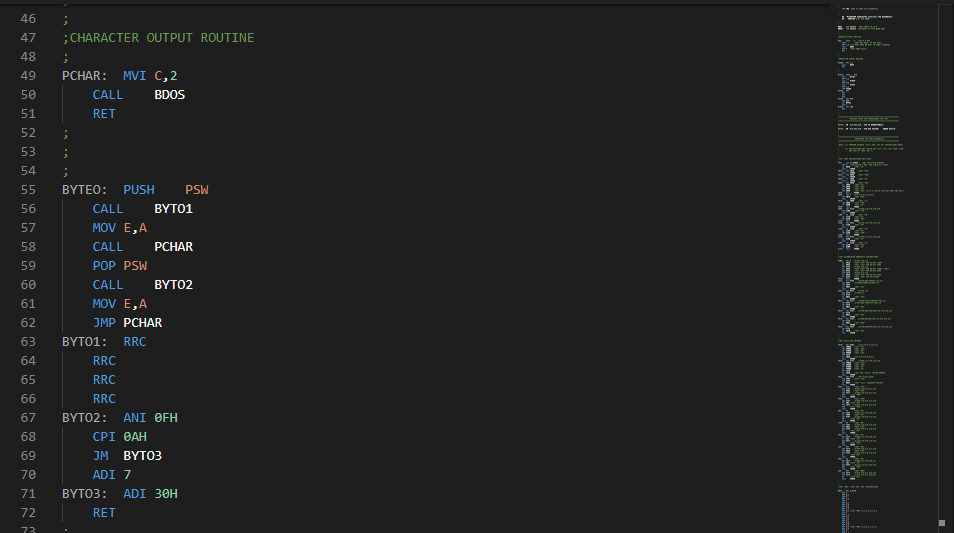
\includegraphics[width=1.0\textwidth]{Bilder/CodeEditor.png}
    \label{fig:codeeditor}
\end{figure}

In Abbildung \ref{fig:codeeditor} sieht man den Code-Editor in Aktion. Die einzelnen Bestandteile des Assembly-Codes, die Labels, die Instruktionen und die Argumente, sowie Kommentare sind alle unterschiedlich eingefärbt.

\begin{figure}
    \caption{Autovervollständigung für Instruktionen}
    \centering
    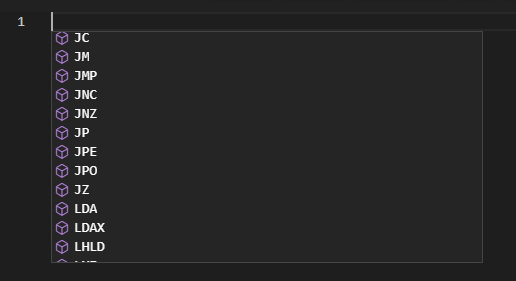
\includegraphics[width=0.6\textwidth]{Bilder/Completion_1.png}
    \label{fig:completion1}
\end{figure}

\begin{figure}
    \caption{Autovervollständigung für Argumente}
    \centering
    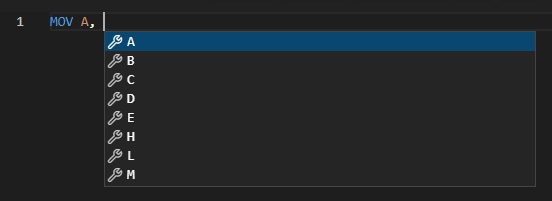
\includegraphics[width=0.6\textwidth]{Bilder/Completion_2.png}
    \label{fig:completion2}
\end{figure}

In den Abbildungen \ref{fig:completion1} und \ref{fig:completion2} sieht man außerdem, wie die Autovervollständigung des Code-Editors funktioniert. Basierend auf der Eingabe des Nutzers und der Position im Code wird automatisch erkannt, ob eine Instruktion oder ein Argument vorgeschlagen wird und welche in Frage kommen.

\subsection{Emulator-Zustand}

Hat der Nutzer nun ein Assembly-Programm mithilfe des Code-Editors erstellt, kann er es auch ausführen lassen. Hierfür wird der in Rust entwickelte Emulator genutzt, der mithilfe der WebAssembly-Schnittstelle in die Webapplikation eingebunden wird. Die Interaktion mit dem Emulator erfolgt mithilfe verschiedener Bedienelemente in einer Aktionsleiste am oberen Rand der Anwendung (siehe Abbildung \ref{fig:actionbar}).

\begin{figure}[h]
    \caption{Aktionsleiste des Emulators}
    \centering
    
\includegraphics[width=0.75\textwidth]{Bilder/Aktionsleiste.png}
    \label{fig:actionbar}
\end{figure}

\begin{figure}
    \caption{\textit{Load}-Dialog}
    \centering
    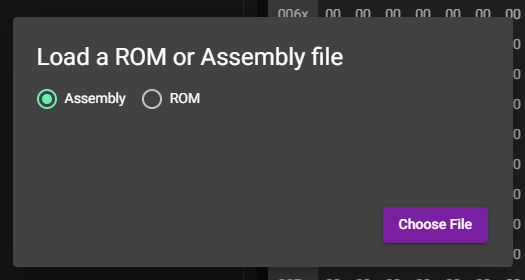
\includegraphics[width=0.75\textwidth]{Bilder/Load_Dialog.png}
    \label{fig:loaddialog}
\end{figure}

Die ersten beiden Schaltflächen der Aktionsleiste, \textit{Load} und \textit{Save}, ermöglichen dem Nutzer, Assemblycode aus Dateien auf seinem Endgerät zu laden oder sie dort zu speichern. \textit{Load} kann außerdem auch bereits assemblierten Code direkt in den Speicher des Emulators laden. Die Auswahl erfolgt mithilfe eines eigenen Auswahldialogs, der in Abbildung \ref{fig:loaddialog} zu sehen ist.

Um den Code, den der Nutzer geschrieben hat, nun zu assemblen, muss dieser in der Aktionsleiste die Funktion \textit{Assemble} nutzen. Ist der Vorgang erfolgreich, werden die Bytes, die der Assembler erzeugt, in den Hauptspeicher des Emulators geschrieben.